\section{Introduction}
\label{sec:intro}

\subsection{A Great Theorem}
The Gauss-Bonnet theorem relates the curvature, a local property, of a surface
to the Euler characteristic, a global property. In symbols 

\begin{equation}\label{eqn:g-b-noboundary}
		\int_MK dA =2\pi \chi(M)
\end{equation}
where $M$ is a smooth surface in $\RR^3$ without bounary, $K$ is Gaussian curvature
and $\chi(M)$ is the Euler characteristic of $M$.
The theorem is a bridge between many ideas that may
seem separate at first, see \figref{bridge}. 




\begin{figure}[htb]
\centering
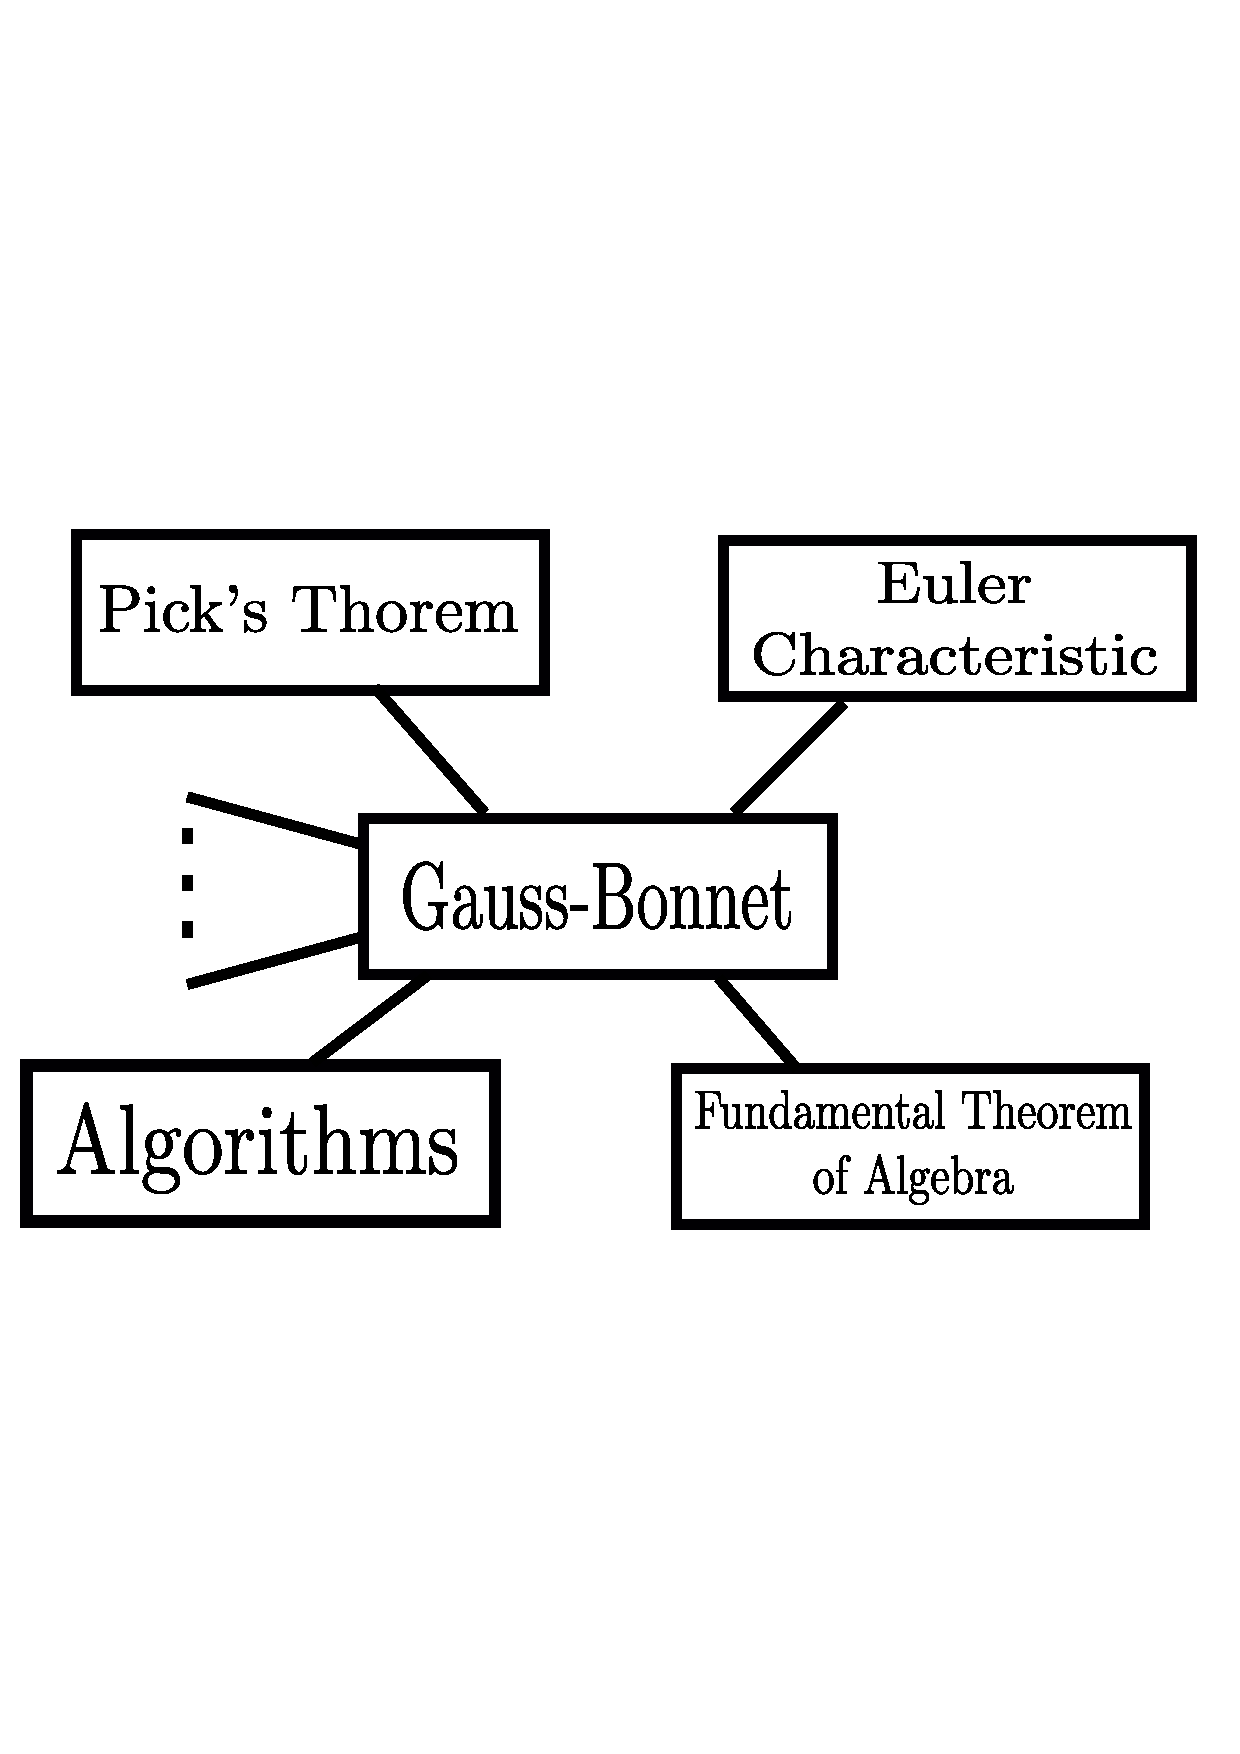
\includegraphics[width=.3\textwidth]{curvature/bridge}
\caption{The Gauss-Bonnet theorem is a star.}
\label{fig:bridge}
\end{figure}

In the book \emph{Using the Borsuk-Ulam Theorem}
\cite{jm08},
Matou\v{s}ek states that a theorem is a great theorem if there are
\begin{enumerate}[(1)]
\item several different equivalent versions,
\item many different proofs,
\item a host of extensions and generalizations, and
\item numerous interesting applications.
\end{enumerate}

By this criteria, the Gauss-Bonnet theorem is a great theorem.
For (1), six\todo{verify} different versions of the theorem are discussed
in \cite{wu_historical_2008}. 
In addition to the version for smooth surfaces given in \eqnref{g-b-noboundary},
we highlight
 several discrete versions for triangulated surfaces. 
  




 
 
As for (2), several fundamentally different proofs exist.  
One common approach is to first prove the theorem for simply connected domains
with boundary, then triangulate a surface and add up the contribution from each triangle.
However, this proof seems to lack a geometric intuition that other proofs provide. \cite{wu_historical_2008},
A second commonly seen proof is to use Stokes theorem  \cite{doc76,pressley_elementary_2010}.
Many other proofs exist \cite{guillemin_differential_2010,levi-bicycle,grinfeld_introduction_2013}.


For (3), the theorem has been generalized in many ways.
The two notable examples are the Chern-Gauss-Bonnet theorem\cite{chern_simple_1944} and
the Atiyah–Singer index theorem is an example  \cite{atiyah_index_1963}.
A generalization to higher dimensions \cite{guillemin_differential_2010}.


As for (4), applications, 
seven are given in \cite{doc76}.
For applications to physics see \cite{tirado-physics-apps,gibbons_applications_2008}.
This work provides many examples related to the algorithms and combinatorics. 
I hope that the number of applications continues to grow,
please share any that you feel
ought to be included\footnote{\text{mccoy2ba@jmu.edu}}.


\subsection{Simple Polygons}
\label{sec:warm-up}

Some of us may remember the following special case
of the Gauss-Bonnet theorem from middle school geometry.
An \EMPH{exterior angle} is created when we extend one of the sides of a polygon.
See \figref{exterior-angles} for an example.
The exterior angle at a vertex can be positive or negative.
If we traverse a polygon and add up the exterior angles
we get $2\pi$ because we perform one revolution.
This is a special case of the Gauss-Bonnet theorem.
No matter how we bend or stretch our polygon,
if the boundary of the polygon stays closed and simple,
the sum the exterior angles will be $2\pi$.

We can also derive a formula for the sum of the angles
of the interior angles.
The proof provides intuition for other proofs we will encounter.
We have
\begin{theorem}\label{thm:triangle}
In the plane, the sum of the interior angles of a triangle is $\pi$.
\end{theorem}
\begin{proof}
Draw a line parallel to one edge through the opposite vertex.
By alternating interior angles in the plane, the sum of the angles
in the triangle equal a straight line.
See \figref{interior-angles} for an example. 
\end{proof}


 \begin{figure}[htb]
         \centering
        \begin{subfigure}[b]{0.35\textwidth}
         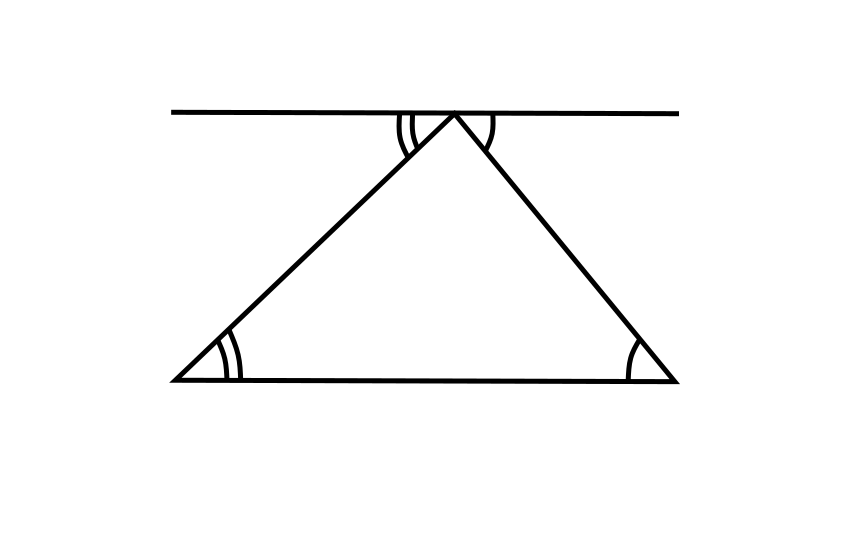
\includegraphics[width=\textwidth]{background/interior-triangle}
         \caption{Interior angles.}
 	 \label{fig:interior-angles}
       \end{subfigure}
         \hspace{1cm}
         \begin{subfigure}[b]{0.25\textwidth}
         \includegraphics[width=\textwidth]{background/exterior-angles-polygon}
         \caption{Exterior angles.}
          \label{fig:exterior-angles}
         \end{subfigure}
		\caption{(a) In the plane, the sum of the interior angles of a triangle is $\pi$
 		and (b) the sum of the exterior angles of a simple
		polygon is $2\pi$. Here
		$\alpha_1+\alpha_2+\alpha_3+\alpha_4+\alpha_5=2\pi$.
 		\label{fig:simple-polygon}}
 \end{figure}

And we have
\begin{corollary}\label{cor:angles}
In the plane, any simple polygon $P$ with $n$ vertices,
the sum of the interior angles of $P$ is $(n-2)\pi$.
\end{corollary}

\begin{proof}
	Consider any simple polygon in the plane $P$ with $n$ vertices. 
	Then $P$ can be triangulated with $n-2$ triangles \cite{orourke_computational_1994}.
	Thus, when we traverse $P$ we go around $n-2$ triangles each contributing
	$\pi$.
\end{proof}

 





On the unit sphere we can determine even more about a polygon 
based on the angles. This is because the sphere is curved.
A triangle on the sphere is shown in \figref{sphere-triangle}.


 \begin{figure}[htb]
         \centering
        \begin{subfigure}[b]{0.35\textwidth}
         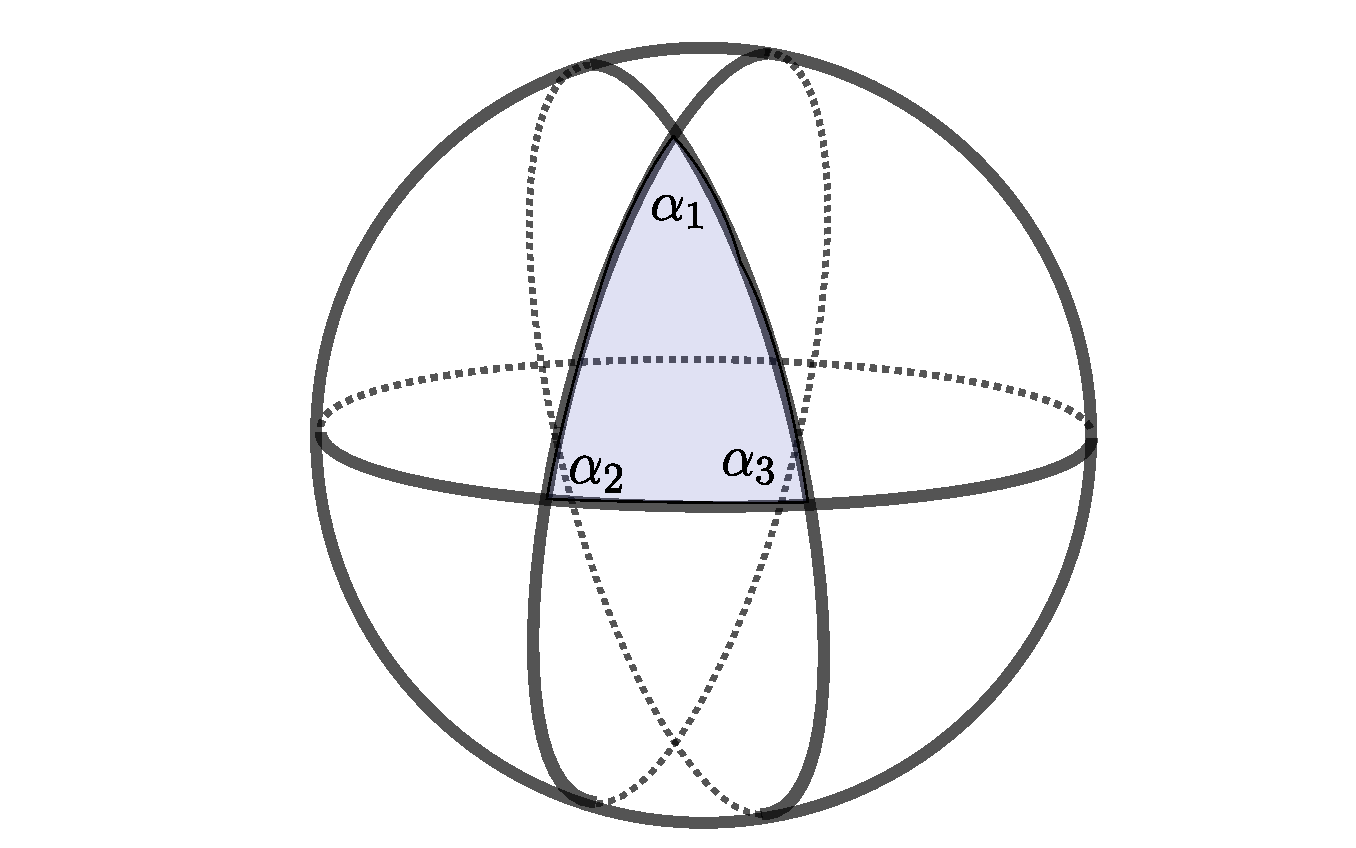
\includegraphics[width=\textwidth]{background/sphere-triangle}
         \caption{Spherical triangle.}
 	 \label{fig:sphere-triangle}
       \end{subfigure}
         \hspace{1cm}
         \begin{subfigure}[b]{0.35\textwidth}
         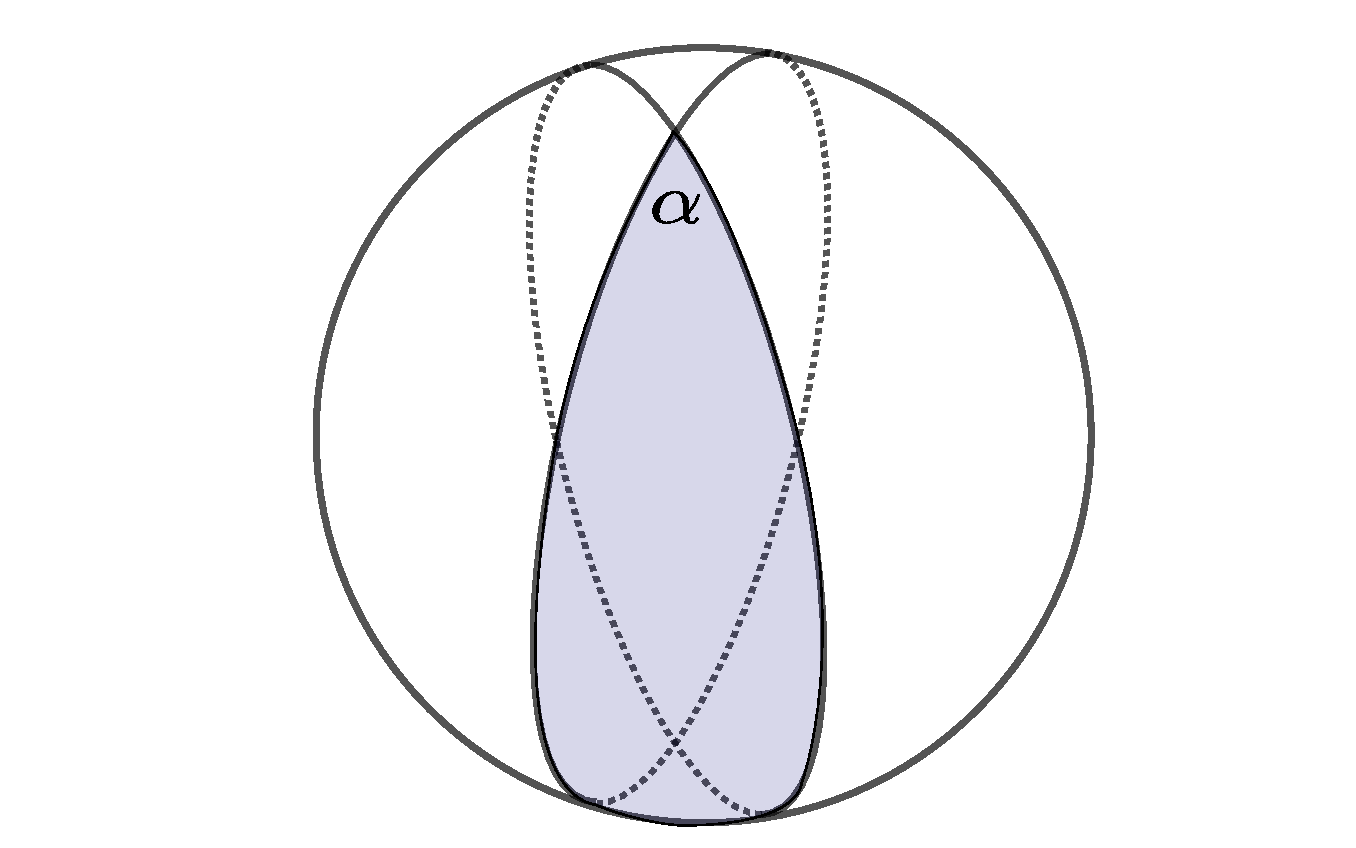
\includegraphics[width=\textwidth]{background/lune}
         \caption{A lune.}
          \label{fig:lune}
         \end{subfigure}
		\caption{(a) A triangle on the sphere.
 		(b) A lune with angle $\alpha$.
 		\label{fig:sphere-lune}}
 \end{figure}
A spherical \EMPH{lune} is the region on a sphere bounded by two half great circles
with angle $\alpha$ the area of a lune is denoted $A(\alpha)$,
 see \figref{lune}.
On the unit sphere, the area of a lune is proportional to $\alpha$. 
If $\alpha=0$ the area is zero and if $\alpha=\pi$ the area is $4\pi$.
We can add the area of two lunes in terms of their angles, 
$A(\alpha_1+\alpha_2)=A(\alpha_1)+A(\alpha_2)$ so $A$ is linear
and  $A(\alpha)=4\alpha.$




The area of a triangle on the sphere is related to the angles.

\begin{lemma}[Area of Spherical Triangle]\label{lem:spherical-triangle}
On the unit sphere, the area of a triangle with interior angles $\alpha_1, \alpha_2, \alpha_3$
is $A=\alpha_1+\alpha_2+\alpha_3-\pi$.
\end{lemma}

\begin{proof}
Any two edges of the the triangle form a lune. The collection of 
all three lunes covers the entire sphere with triangle and the antipodal triangle
are covered three times. The surface area of the unit sphere is $4\pi$.

Thus, $4\pi=2(2\alpha_1+2\alpha_2+2\alpha_3)-6A+2A$
and $A=\alpha_1+\alpha_2+\alpha_3-\pi$.
\end{proof}

As in the plane, any polygon on the sphere with $n$ vertices can be decomposed
into $n-2$ triangles. This gives a formula for the area of a simple polygon
on the sphere with interior angles $\beta_1,\beta_2,\ldots, \beta_n$.

\begin{equation} \label{eqn:sphere-area}
A=(2-n)\pi +\sum_{i=1}^n \beta_i.
\end{equation}







\subsection{Pick's Theorem}
\label{sec:pick}

Pick's Theorem gives a formula for the area of a polygon
in the plane with vertices on the lattice $\ZZ^2$ \cite{og-pick}.
We give a proof originally due to Blatter \cite{blatter_another_1997}
and restated by Tabachnikov  \cite{tabachnikov_proofs_2014}.

\begin{theorem}[Pick's Theorem]\label{thm:pick}
Let $P$ be a simple polygon in the plane with vertices on the lattice $\ZZ^2$,
let $I$ be the number of lattice points inside of $P$, let $B$ be the number
of lattice points on the boundary of $P$ and let $A$ denote the area of $P$.
Then, 
$$A=I+\frac{B}{2}-1.$$
\end{theorem}
See \figref{picks} for an example.

 \begin{figure}[htb]
         \centering
         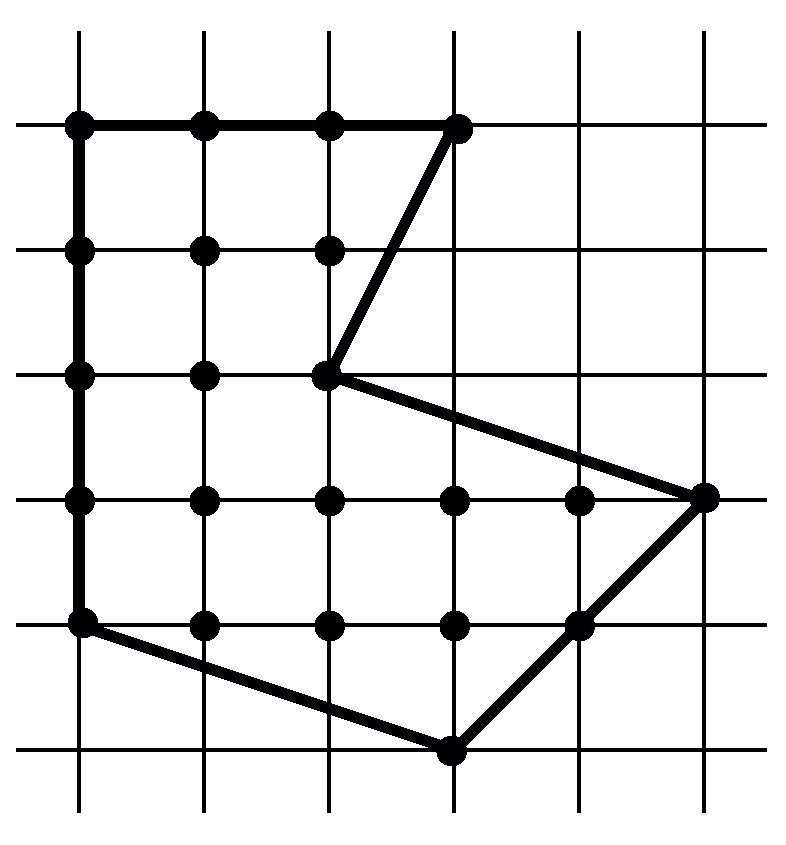
\includegraphics[width=5cm]{pick}
	\caption{A polygon with vertices on the lattice. 
	There are 10 interior vertices and 12 vertices on the boundary.
	By Pick's theorem the area of the polygon is $10+\frac{12}{2}-1=15.$
	\label{fig:picks}}
 \end{figure}
 
\begin{proof}
	Put a unit volume ice cube at each lattice point in the plane and let the ice melt.
	The water will evenly cover the plane with the amount of water inside the polygon 
	equal to its area.
	
	Consider a edge on the the polygon. The amount of water that flows
	into to polygon across this edge equals that amount of water that flows out of the polygon
	across this edge by symmetry. 
	So, the total flow across each edge is zero and
	the  amount of water inside the polygon comes from interior cubes and the lattice vertices
	of the polygon.
	
	Each interior lattice point contributes one unit of water. 
	Each lattice point on an edge, half of the water flows into the polygon and
	half flows outside of the polygon.
	Let $\alpha_i$ denote the interior angles at each vertex.
	Each vertex contributes $\frac{\alpha_i}{2\pi}$ units of water to the area.
	By the Gauss-Bonnet theorem, \thmref{simple-bonnet}, the sum of the interior
	angles is $\pi(n-2)$. Thus, the vertex points contribute a total of 
	$$\frac{\pi(n-2)}{2\pi}=\frac{n}{2}-1.$$
	The theorem follows.

\end{proof}




